\documentclass[conference,a4paper]{IEEEtran}

% *** GRAPHICS RELATED PACKAGES ***
%
\ifCLASSINFOpdf
   \usepackage[pdftex]{graphicx}
\else
  % or other class option (dvipsone, dvipdf, if not using dvips). graphicx
  % will default to the driver specified in the system graphics.cfg if no
  % driver is specified.
  \usepackage[dvips]{graphicx}
\fi

\usepackage[cmex10]{amsmath}
\interdisplaylinepenalty=2500

\usepackage[font=footnotesize]{subfig}
\usepackage{algorithm}
\usepackage{algorithmic}
\usepackage{float}
\newfloat{algorithm}{t}{lop}
\usepackage{amssymb}
\usepackage{hyperref}  % Needed by Pandoc
\usepackage{longtable} % Needed by Pandoc
\usepackage{booktabs}  % Needed by longtable fix

\usepackage{amsthm}
\newtheorem{theorem}{Theorem}[section]
\newtheorem{proposition}[theorem]{Proposition}

% correct bad hyphenation here
\hyphenation{op-tical net-works semi-conduc-tor}

%Nic:
\providecommand{\abs}[1]{\lvert#1\rvert}
\providecommand{\norm}[1]{\lVert#1\rVert}

% Fix for the longtable envirnoment generated by Pandoc
% from here http://tex.stackexchange.com/questions/161431/how-to-solve-longtable-is-not-in-1-column-mode-error/224096#224096
% Other possible solutions: see https://github.com/jgm/pandoc/issues/1023
\makeatletter
\let\oldlt\longtable
\let\endoldlt\endlongtable
\def\longtable{\@ifnextchar[\longtable@i \longtable@ii}
\def\longtable@i[#1]{\begin{figure}[t]
\onecolumn
\begin{minipage}{0.5\textwidth}
\oldlt[#1]
}
\def\longtable@ii{\begin{figure}[t]
\onecolumn
\begin{minipage}{0.5\textwidth}
\oldlt
}
\def\endlongtable{\endoldlt
\end{minipage}
\twocolumn
\end{figure}}
\makeatother


\begin{document}

\title{Greedy Least Squares Pursuit for sparse signal recovery}


\author{
  \IEEEauthorblockN{Nicolae Cleju}
  \IEEEauthorblockA{Faculty of Electronics, Telecommunications and Information Technology\\
``Gheorghe Asachi'' Technical University of Iasi\\
700506, Iasi, Romania\\
Email: \{nikcleju\}@etti.tuiasi.ro}
}

\maketitle

\begin{abstract}
Abstract goes here. You can write it on multiple lines, and it can
contain equations like \(a = b\).
\end{abstract}

\IEEEpeerreviewmaketitle


\section{Introduction}\label{sec:intro}

We are in section \ref{sec:intro}.

Here is a reference {[}1{]}. So far so good.

Some equation is presented in (\ref{eq:eq1}) below:
\begin{equation}x = 1 + 2\label{eq:eq1}\end{equation}

A nice image is in Fig.~\ref{fig:test}.

\begin{figure}
\centering
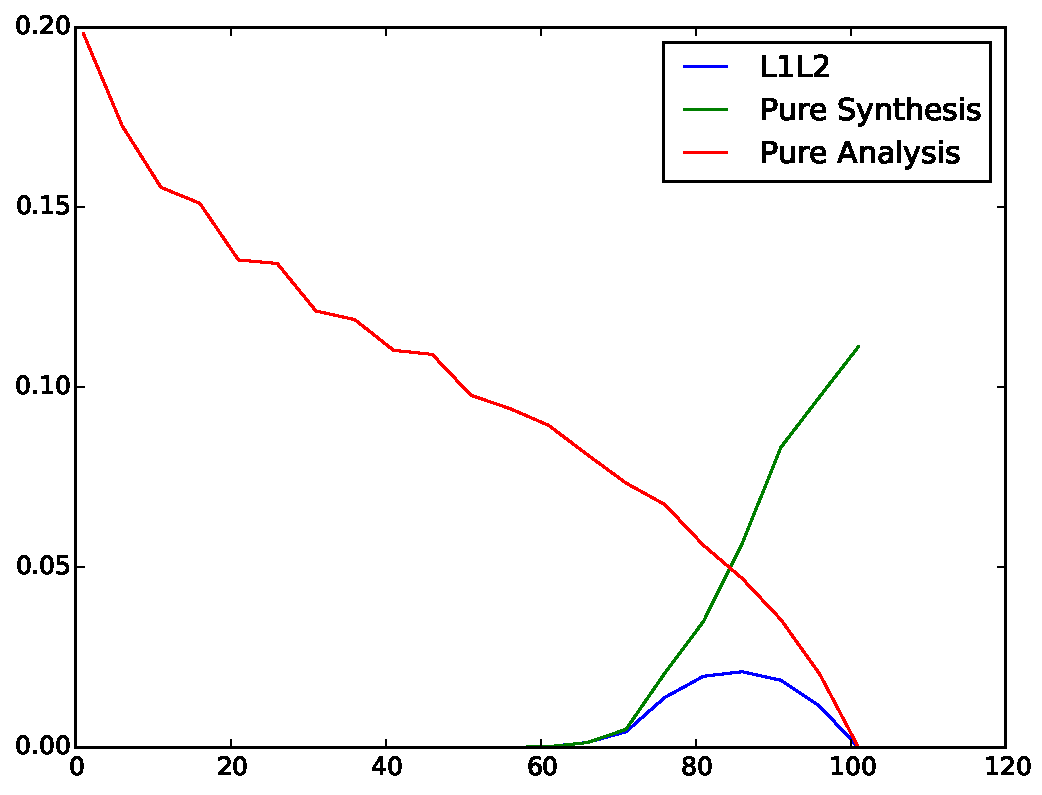
\includegraphics[width=0.40000\textwidth]{Figure.pdf}
\caption{Nume figura}\label{fig:test}
\end{figure}

We can also have a nice looking table, Table~\ref{tbl:simple}. Just keep
it small, you may get problems if it is larger than one page.

\hypertarget{tbl:simple}{}
\begin{longtable}[]{@{}rlcl@{}}
\caption{\label{tbl:simple}Demonstration of simple table syntax.
}\tabularnewline
\toprule
Right & Left & Center & Default\tabularnewline
\midrule
\endfirsthead
\toprule
Right & Left & Center & Default\tabularnewline
\midrule
\endhead
12 & 12 & 12 & 12\tabularnewline
123 & 123 & 123 & 123\tabularnewline
1 & 1 & 1 & 1\tabularnewline
\bottomrule
\end{longtable}

\section*{References}\label{references}
\addcontentsline{toc}{section}{References}

\hypertarget{refs}{}
\hypertarget{ref-Cleju2011ISSCS}{}
{[}1{]} N. Cleju, C. M. Fira, C. Barabasa, and L. Goras, ``Robust
reconstruction of compressively sensed ECG signals,'' in \emph{Proc.
isscs 2011}, 2011, pp. 507--510.

%\bibliographystyle{IEEEtran}
%\bibliography{IEEEfull,MyJfull,Biblio}

\end{document}


